% ****** Start of file template-TIF360-FYM360-blindtext.tex ******
%
% use on Overleaf!!!!
%
\documentclass[%
 reprint,
 amsmath,amssymb,
 aps,
]{revtex4-2}

\usepackage{subcaption} % Essential for subfigure environment


\usepackage{graphicx}% Include figure files
\usepackage{dcolumn}% Align table columns on decimal point
\usepackage{bm}% bold math
\usepackage{hyperref}% add hypertext capabilities
%\usepackage[mathlines]{lineno}% Enable numbering of text and display math
%\linenumbers\relax % Commence numbering lines
\usepackage{xcolor}

\usepackage{lipsum}

\begin{document}

\title{AI for Three-Body Problem Trajectory Classification: \\
A Comparative Study of TCN, Reservoir and LSTM}

\author{Esben Almkvist}


\date{\today}% It is always \today, today,
             %  but any date may be explicitly specified

\begin{abstract} %%% DO NOT CHANGE!
%%% - B1 - %%%%%%%%%%%%%%%%%%%%%%%%%%%%%%%%%%% 
%%% Customize this part: text between - B1 - and - E1 - must not appear in the final report 
\noindent The three-body problem stands as a classic example of chaos theory, representing perhaps the simplest physical system that exhibits chaotic behavior. In this study, the three-body problem is simulated in two dimensions and machine learning models to predict its dynamics are developed. Multiple approaches are explored, including one-dimensional temporal convolutional networks (TCN), basic long-short-term memory (LSTM) networks, and reservoir models. The Reservoir models trained very fast and produced the best results for short forecasts, while the TCN performed best for longer forecasts.  

\begin{itemize}
    \item Abstract: Classic three body problem. Create simulation data with physical model and train and forecast using three different neural network models. Predict trajectories. Three models. Classic RNN LSTM and Specialized TCN, and Reservoir. The latter two performed best. The TCN would predic the general trajectories accurate, but not the interaction of the bodies.
\end{itemize}

%%% - E1 - %%%%%%%%%%%%%%%%%%%%%%%%%%%%%%%%%%%%%%

\begin{description} %%% DO NOT CHANGE!
\item[Project Topic] %%% DO NOT CHANGE!
{Project K\\
Three Bodies, Three Models: Chaotic Time Series Analysis with Machine
Learning.} %CHANGE accordingly
\item[Teaching Assistant] %%% DO NOT CHANGE!
{Alex Lech} % CHANGE accordingly
\end{description} %%% DO NOT CHANGE!
\end{abstract}

\maketitle




\section{\label{sec:intro}Introduction} %%% DO NOT CHANGE!

%%% - B2 - %%%%%%%%%%%%%%%%%%%%%%%%%%%%%%%%%%% 
%%% Customize this part: text between - B2 - and - E2 - must not appear in the final report 
The prediction of chaotic systems remains a major challenge in both physics and machine learning due to their sensitivity to initial conditions \cite{grebogi1983final}. Time series forecasting have traditionally used recurring neural networks (RNNs) as best practice \cite{vlachas2018data}, but recently several other approaches have proved capable to match the performance of the RNNs. In particular, reservoir computing (RC) has emerged as a compelling model-free strategy \cite{pathak2018model}, offering the ability to learn temporal dynamics directly from data without requiring prior knowledge of the system's governing equations. One-dimensional convolutional neural networks often outperform canonical recurrent networks such as LSTMs \cite{bai2018empiricalevaluationgenericconvolutional}. 
This has important implications for high-dimensional systems like turbulent flows \cite{Pandey_PhysRevFluids.5.113506} and multiscale climate dynamics \cite{Chattopadhyay2019}.

In the work of Pathak et al. \cite{pathak2018model} it was demonstrated that RC could accurately forecast the evolution of complex systems over short time horizons. While classical neural networks like LSTM also offer predictive capabilities \cite{vlachas2018data}, their interpretability and training demands are often less 
favorable compared to RC \cite{Kobayashi_PhysRevE.104.044215}. No literature was found where the Three body problem was forecasted using neural network models, but several studies looked at the Lorenz attractor as a proxy for testing the skills of weather forecasting \cite{Chattopadhyay2019, vlachas2018data}.
In this project, we test three methods: LSTM, TCN and RC to the Three body problem, assess their forecasting skill, and discuss the limitations and potential for generalization.

\begin{itemize}
    \item Introduction: Three body problem is not refered to in previous studies of neural networks. Probably because of its chaotic behavior and disruptive behavior when bodies collide or escape. When two or all three objects are very close and the distance approaches zero, the gravitation becomes very large and an object is often catapulted out of the system; at least when simulated with a finite time step. A more common approach is using the Lorenz system to simulate a chaotic system that resembles natural phenomena, such as weather.
\end{itemize}


%% Get a better citation than Kobayashi

%%% - E2 - %%%%%%%%%%%%%%%%%%%%%%%%%%%%%%%%%%%%%%






\section{\label{sec:overview}Overview} %%% DO NOT CHANGE!

%%% - B3 - %%%%%%%%%%%%%%%%%%%%%%%%%%%%%%%%%%% 
%%% Customize this part: text between - B3 - and - E3 - must not appear in the final report 
Recent literature suggests various data-driven models capable of forecasting chaotic time series. Each method varies in complexity, interpretability, and performance depending on the task. 

\begin{table*}
    \caption{\textbf{Overview of time-series forecasting methods for chaotic systems.} Summary of commonly used methods, their features, and suitability.}
    \label{tab:methodsoverview}
    \begin{tabular}{|p{2cm}|p{3cm}|p{6cm}|p{6cm}|}
    \hline
       \textbf{Method}  &  \textbf{Use case scenario}   &  \textbf{Features}  &  \textbf{Suitable for the project?}   \\
    \hline
        Reservoir Computing (RC)  & Chaotic time-series forecasting & Simple training; good short-term prediction; low interpretability; sensitive to hyperparameters \cite{pathak2018model, Pandey_PhysRevFluids.5.113506} & Yes. Best balance of performance and efficiency for model-free prediction.  \\
    \hline
        Long Short-Term Memory (LSTM) & High-dimensional spatiotemporal systems & Capable of long-term memory; data-hungry; harder to interpret \cite{vlachas2018data} & Moderate. Selected as a standard model used for timeseries forecasting.  \\
    \hline
        TCN & Chaotic and multiscale time series & Good for sequence modeling with long memory and parallel computation; interpretable; requires careful tuning \cite{bai2018empiricalevaluationgenericconvolutional} & Yes. Offers complementary strengths to RC and LSTM for medium- to long-term forecasting. \\
    \hline
        PINN & Nonlinear partial differential equations & A promising methodology is Physics-informed neural networks (PINN) \cite{RAISSI2019686}, which could be used as an alternative to forecasting the system. & No. Since the simulated system was not physically sound as the energy was not conserved. \\
    \hline
    \end{tabular}
\end{table*}

Given the trade-offs, the first three methods were implemented and evaluated: RC, LSTM, and TCN, to explore their comparative strengths in forecasting the three-body problem. The PINN method was selected given that the time step was such that energy was not conserved in the simulated system. 

\begin{itemize}
    \item Overview:   When simulating time series using neural networks a classical approach is to use RNNs as they are good at capturing recurring phenomena. Therefore a LSTM was used to represent the classical method for time series forecasting. In recent years 1D CCNs have been used to forecast time series with success, often performing better than traditional RNN methods. A modern TCN was used as the second model. Reservoir models have proven to be good at predicting the behavior of chaotic systems, so that was chosen as the third model.
\end{itemize}


%%% - E3 - %%%%%%%%%%%%%%%%%%%%%%%%%%%%%%%%%%%%%%




\section{\label{sec:method}Method} %%% DO NOT CHANGE!

%%% - B4 - %%%%%%%%%%%%%%%%%%%%%%%%%%%%%%%%%%% 
%%% Customize this part: text between - B4 - and - E4 - must not appear in the final report 
Three methods were adapted for use to predict the future state of the Three body problem. A vanilla version of LSTM with two layers with a hidden dimension of 256 neurons was used as a standard approach for time series modeling. 
For TCN, a three layer model with [256, 512, 256] neurons was used.
We use Echo State Networks (ESNs), a class of reservoir computers, for model-free forecasting. The input time series is fed into a randomly initialized and fixed recurrent neural network (the reservoir), producing a dynamic state vector. The final output is generated by a linear readout layer trained via ridge regression.

Mathematically, the reservoir state $\mathbf{r}(t)$ evolves as:
\begin{equation}
\mathbf{r}(t+1) = \tanh(\mathbf{W}_{\text{in}}\mathbf{u}(t) + \mathbf{W}\mathbf{r}(t)),
\end{equation}
where $\mathbf{W}_{\text{in}}$ and $\mathbf{W}$ are the input and recurrent weight matrices, respectively. The output is:
\begin{equation}
\hat{\mathbf{y}}(t) = \mathbf{W}_{\text{out}}\mathbf{r}(t).
\end{equation}

The training involves optimizing $\mathbf{W}_{\text{out}}$ to minimize the mean squared error between $\hat{\mathbf{y}}(t)$ and the target $\mathbf{y}(t)$.


    \begin{enumerate}
        \item \textbf{Data Generation}
        \begin{itemize}
            \item Simulated multiple 2D three-body systems with varying initial conditions with Newtonian gravity and numerically integrated motion using the \textbf{Leapfrog method}.
            \item Each simulation was labeled as: 
            \begin{itemize}
                \item \texttt{converging}: Collision occurs when the distance between the two bodies is less than or equal to the sum of their radii.
                \item \texttt{diverging}: Escape energy is greater than $\varepsilon$, which was set to 2 J: \[
                \underbrace{\frac{1}{2}m_i v_i^2}_{\text{Kinetic Energy}} \underbrace{-\sum_{i \ne j} \frac{G m_i m_j}{r_{ij}}}_{\text{Potential Energy}} > \varepsilon
                \] 
                \item \texttt{stable}: When the system simulated 800 time steps of 0.01 seconds without any of the bodies escaping or colliding.
            \end{itemize}
        \end{itemize}
    \begin{figure}
        \centering
            \begin{minipage}{0.15723\textwidth}
                \centering
                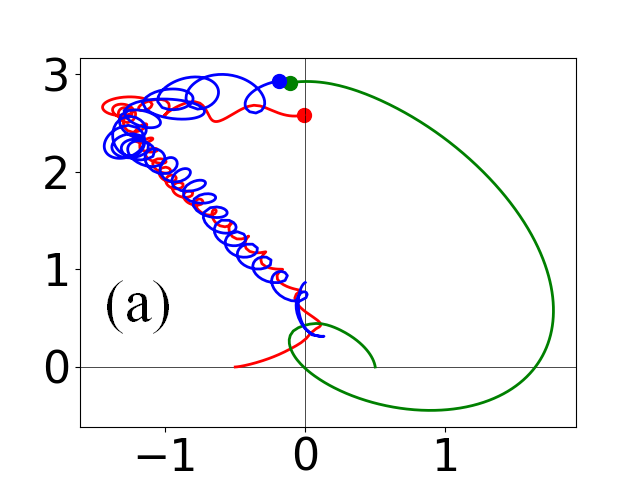
\includegraphics[width=\linewidth]{threebodies_15_marked.png}
            \end{minipage}
            \hfill
            \begin{minipage}{0.15723\textwidth}
                \centering
                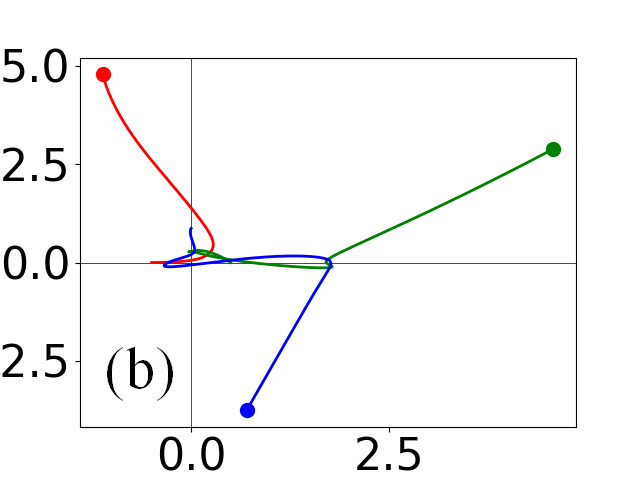
\includegraphics[width=\linewidth]{threebodies_14_marked.png}
            \end{minipage}
            \hfill
            \begin{minipage}{0.15723\textwidth}
                \centering
                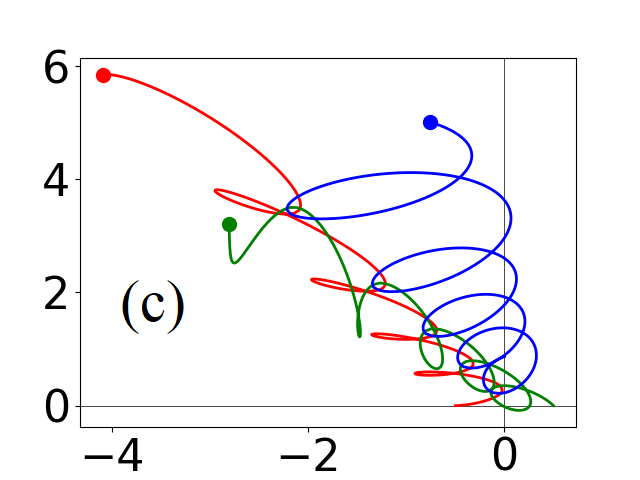
\includegraphics[width=\linewidth]{threebodies_13_marked.png}
            \end{minipage}
    
        \caption{\textbf{Three body simulation.} The simulated trajectories for the three bodies for the different classes (a) converging, (b) diverging and (c) stable.}
        \label{fig:classes}    
    \end{figure}
                
    \item \textbf{Data Preparation}
        \begin{itemize}
            \item Extracted time series of positions and velocities for all three bodies.
            \item Created sequence windows of 200 time steps for training and 600 time steps for prediction.
        \end{itemize}
    
        \item \textbf{Modeling Approaches}
        \begin{itemize}
            \item \textbf{LSTM}: Used hidden dimension of 256 and weighted loss depending on forecast horizon.
            \item \textbf{TCN}: Used five layers with [128, 256, 512, 256, 128] neurons and the same weighted loss function as for LSTM.
            \item \textbf{Reservoir Computing}: Used a  reservoir size of 1750 and set input parameters to avoid overfitting and instability.
        \end{itemize}
\end{enumerate}

\begin{itemize}
    \item Method: Describe data generation and selecting stable, converging and diverging systems. Show and describe the figures. 800 steps maximum. Input sequence length and forecasting 600 time steps. Also tested a regressive method, only forecasting one timestep and forecasting the next step based on the forecasted data. This was abandoned as the forecasting in one go performed better. Describe each neural network method and the theory of each. Initially the idea was to predict the trajectories of the objects and then, based on the trajectories, check if the objects would collide, escape or remain stable. However, due to three reasons, the study focuses on predicting the trajectories of the objects rather than classifying the outcome: Simulation length. When objects collide or escape, the simulation was terminated giving it a length shorter than that of the stable case. For the system to learn properly, it was better to use longer sequences of data, which would favor the stable case. The models did not perform well enough for a meaningful classification based on the trajectories. When the bodies passed very close, the difference between a collision and escape due to the catapulting effect was well below the accuracy of the models. Only the stable sequences with 800 time steps were chosen train the neural network models. The Lyapunov time was calculated to relate the time to other chaotic systems and natural phenomena. Figure shows the Lyapunov lambda and time. A Model Time Unit (MTU) was calculated. The energy should be conserved in the system, so to see how it behaved, it was calculated for the simulation and for the neural network models.
\end{itemize}


%%% - E4 - %%%%%%%%%%%%%%%%%%%%%%%%%%%%%%%%%%%%%%





\section{\label{sec:results}Results and Discussion} %%% DO NOT CHANGE!

%%% - B5 - %%%%%%%%%%%%%%%%%%%%%%%%%%%%%%%%%%% 
%%% Customize this part: text between - B5 - and - E5 - must not appear in the final report 
Defining the Lyapunov time. As shown in figure \ref{fig:lyapunov}, the fitted line gives a Lyapunov time for the simulations of 2.49 seconds. This is analogous to about 2 days in weather forecasting, thus forecasting more than 10 seconds will lead to unstable results. In this case, as we trained the model on 200 time steps (2 seconds) and simulated 600 time steps (6 seconds), we are within the time frame of stability of the system.

Figure~\ref{fig:reservoir} shows the RC-based prediction of the three body system. The forecast remains accurate for several Lyapunov times before diverging, consistent with previous observations \cite{pathak2018model}.

\begin{itemize}
    \item Results and Discussion: Describe what is in the figures. The LSTM did not learn much of the system's behavior. The TCN was good at predicting the long term movement of the trajectories. The reservoir was able to predict the behavior of the bodies quite well, but would go wrong more often than the TCN in the long run. By combining the TCN to predict the development of the system and reservoir to predict the residuals to mimic the behavior of the bodies, one could get higher accuracy. The table shows that the TCN and reservoir perform much better than the LSTM. The figures show that two regimes, one where all three bodies interact with each other and one where two bodies circulate around each other while the third body is in its own orbit. This last behavior was often well predicted as to the general direction of the bodies, but the interaction between the bodies was only captured by the reservoir model. The energy was not conserved properly in the simulation due to a too large time step.
    \item Another approach could be to train the model to predict the positional change in each time step instead of the position itself. The distance to the other objects could also be used to make sure that the model will understand that something occurs when two bodies are close. As the simulation was stopped when two bodies collided or when the escape energy was large enough to escape, which occurred just after a close encounter of two or all three bodies, the model would never learn that the bodies are catapulted away during such occasions.
\end{itemize}


\begin{figure}
    \centering
            \begin{minipage}{0.2333\textwidth}
                \centering
                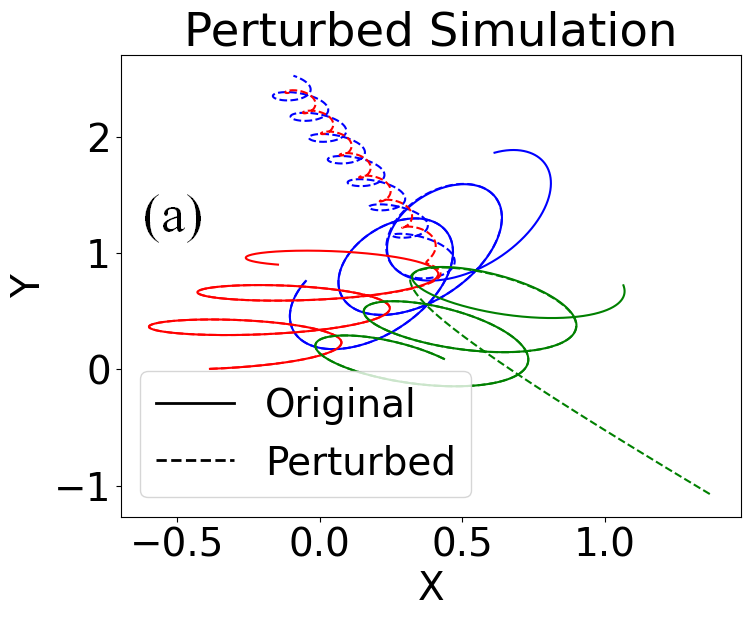
\includegraphics[width=\columnwidth]{Lyapunov_x_y_simulation_marked.png}
            \end{minipage}
            \hfill
            \begin{minipage}{0.2427\textwidth}
                \centering
                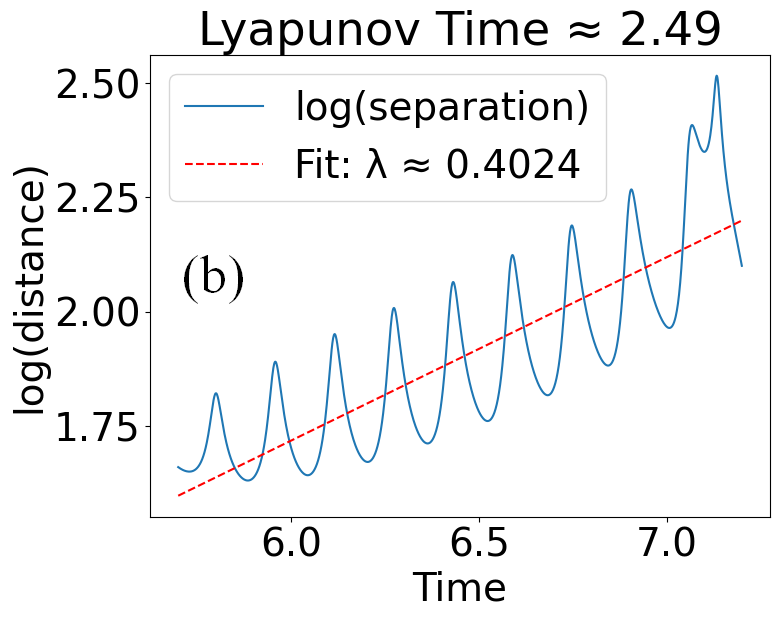
\includegraphics[width=\columnwidth]{Lyapunov_time_marked.png}
            \end{minipage}
    
    \caption{\textbf{Lyapunov time calculation.} The Lyapunov time was calculated for a period when the log of the separation was linear.(a) Position perturbed by $10^{-8}$ in the simulation. (b) Linear fitting to log of separation.}
    \label{fig:lyapunov}
\end{figure}

\begin{figure*}[htbp] % [htbp] is a common placement preference (here, top, bottom, page)
    \centering
    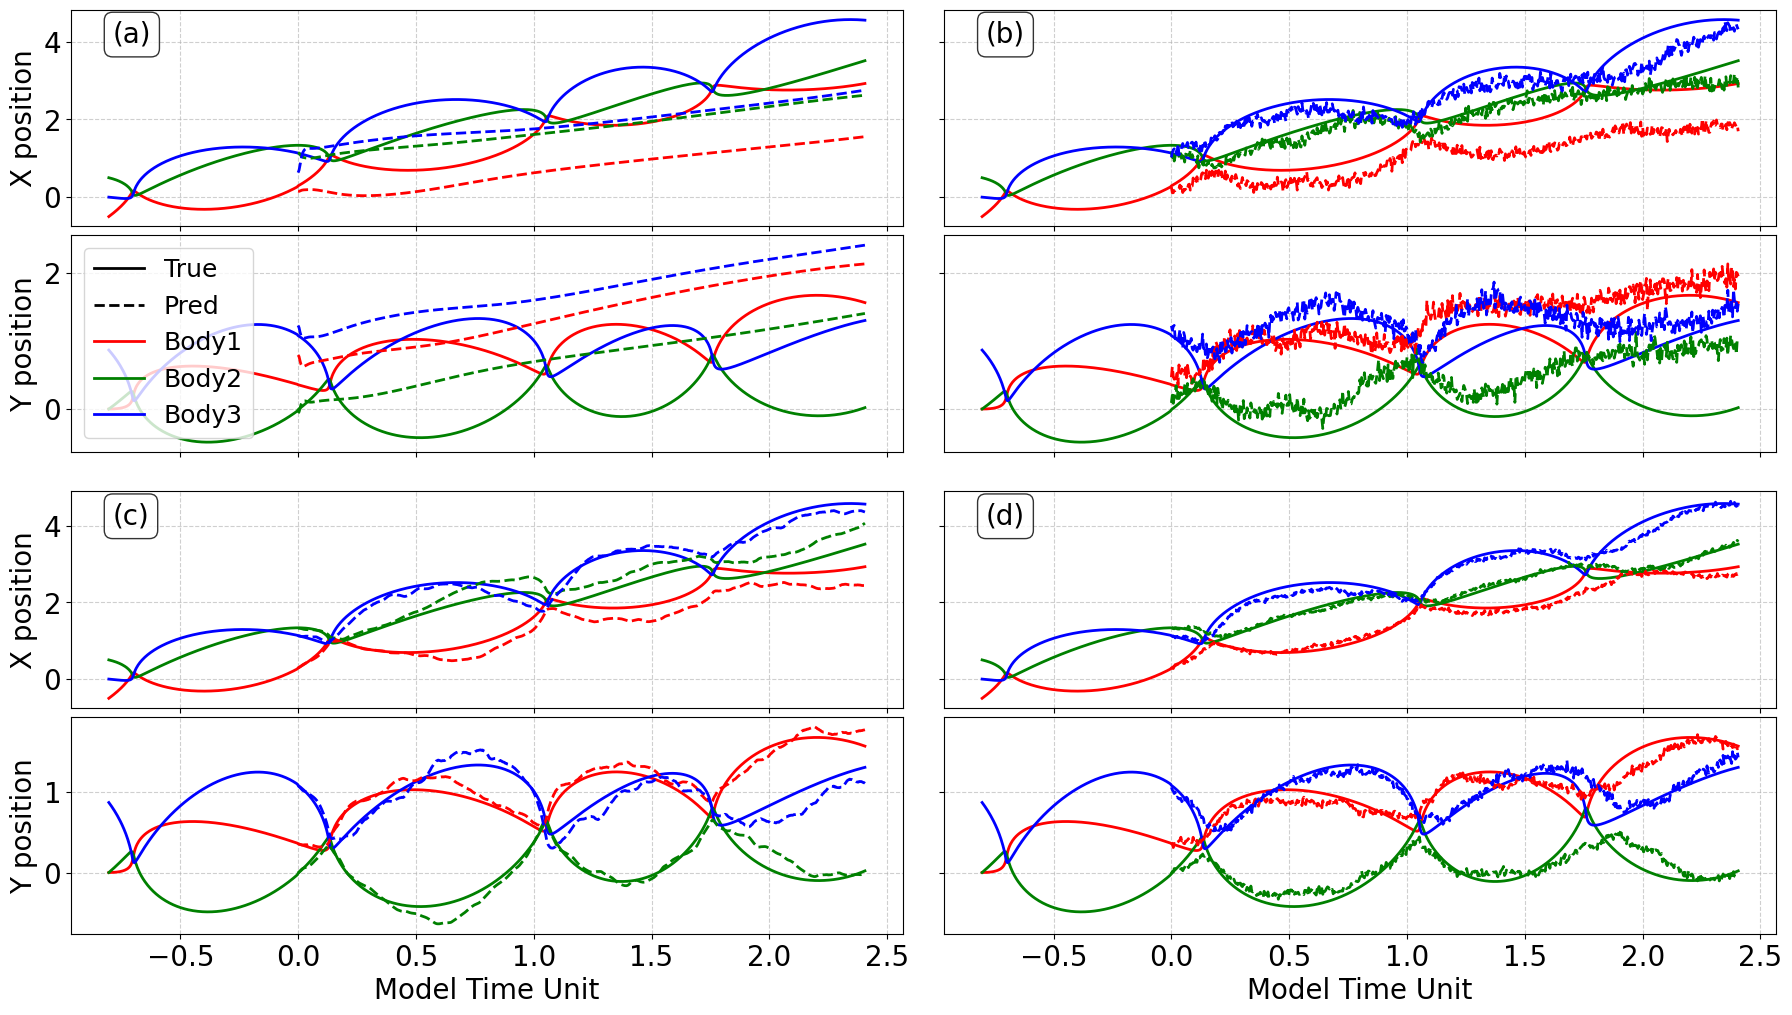
\includegraphics[width=\linewidth]{plot_1_Final_Allplots_22x12_v2.png}
    \caption{Performance of different models for Prediction Set 1. (a) LSTM, (b) TCN, (c) Reservoir Computing, and (d) Combined Model.}
    \label{fig:prediction_set_1_results}
\end{figure*}


\begin{figure*}[htbp]
    \centering
    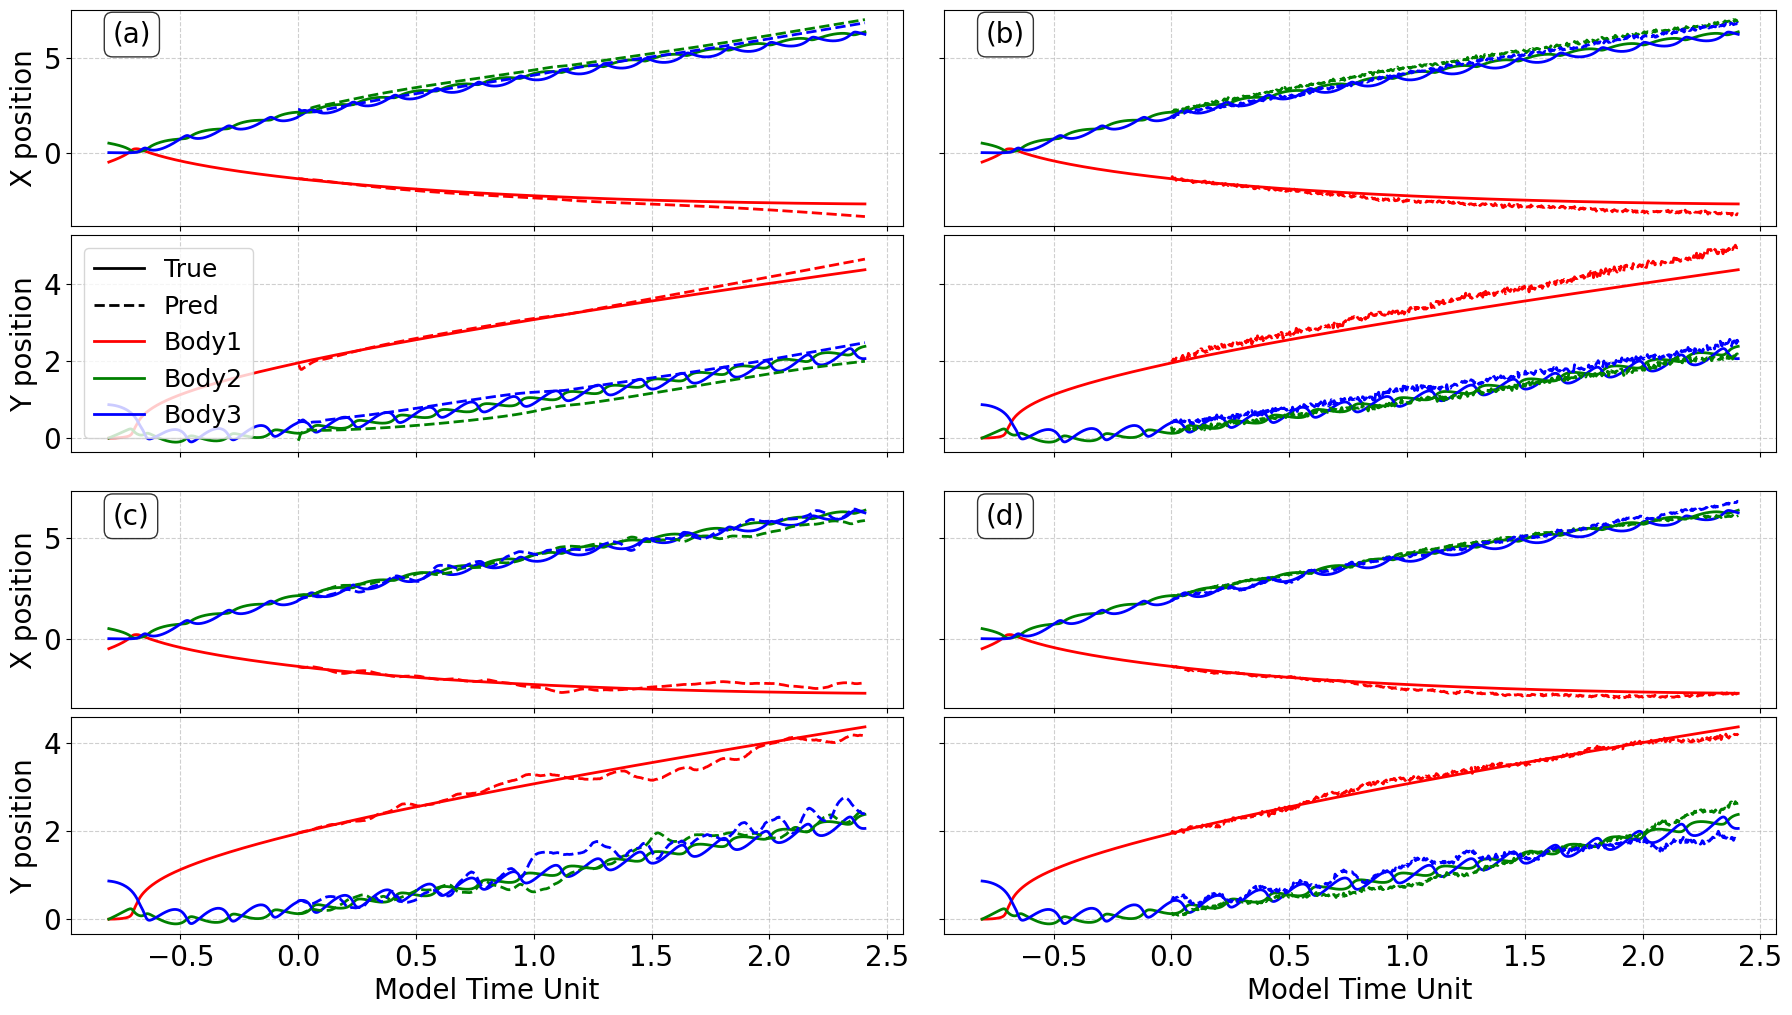
\includegraphics[width=\linewidth]{plot_3_Final_Allplots_22x12_v2.png}
    \caption{Performance of different models for Prediction Set 2. (a) LSTM, (b) TCN, (c) Reservoir Computing, and (d) Combined Model.}
    \label{fig:prediction_set_2_results}
\end{figure*}

Figure~\ref{fig:reservoir} quantifies the error growth. Despite initial accuracy, predictability is fundamentally limited \cite{grebogi1983final}. Still, RC successfully captures short-term dynamics and underlying structure.

\begin{itemize}
\item Only one type of model achieved reasonable performance on forecasts, \textbf{Reservoir models}.
\item \textbf{LSTM} had trouble learning to forecast long forecasts.
\item \textbf{TCN} performed quite well when forecasting long forecasts, but had trouble with shorter forecasts and had a lot of noise.
\item \textbf{Reservoir models} trained fastest and achieved the best accuracy.
\end{itemize}

\iffalse
\begin{figure*}
    \centering
    \includegraphics[width=0.497\linewidth]{plot_1_Lyapunov_LSTM.png}
    \includegraphics[width=0.497\linewidth]{plot_2_Lyapunov_LSTM.png}
    \caption{\textbf{LSTM:} The models are able to predict the general direction of the bodies, but have trouble simulating the behavior of the system.}
    \label{fig:lstm}
\end{figure*}

\begin{figure*}
    \centering
    \includegraphics[width=0.497\linewidth]{plot_1_Lyapunov_TCN.png}
    \includegraphics[width=0.497\linewidth]{plot_3_Lyapunov_TCN.png}
    \caption{\textbf{TCN:} The forecasts are jagged compared to the other model types, probably due to the number of layer. The model captures the general behavior of the system.}
    \label{fig:tcn}
\end{figure*}

\begin{figure*}
    \centering
    \includegraphics[width=0.497\linewidth]{plot_1_Lyapunov_Reservoir.png}
    \includegraphics[width=0.497\linewidth]{plot_3_Lyapunov_Reservoir.png}
    \caption{\textbf{Reservoir:} The model captures the behavior of the bodies quite well, even after several 100 time steps.}
    \label{fig:reservoir}
\end{figure*}
\fi

\begin{figure*}
    \centering
    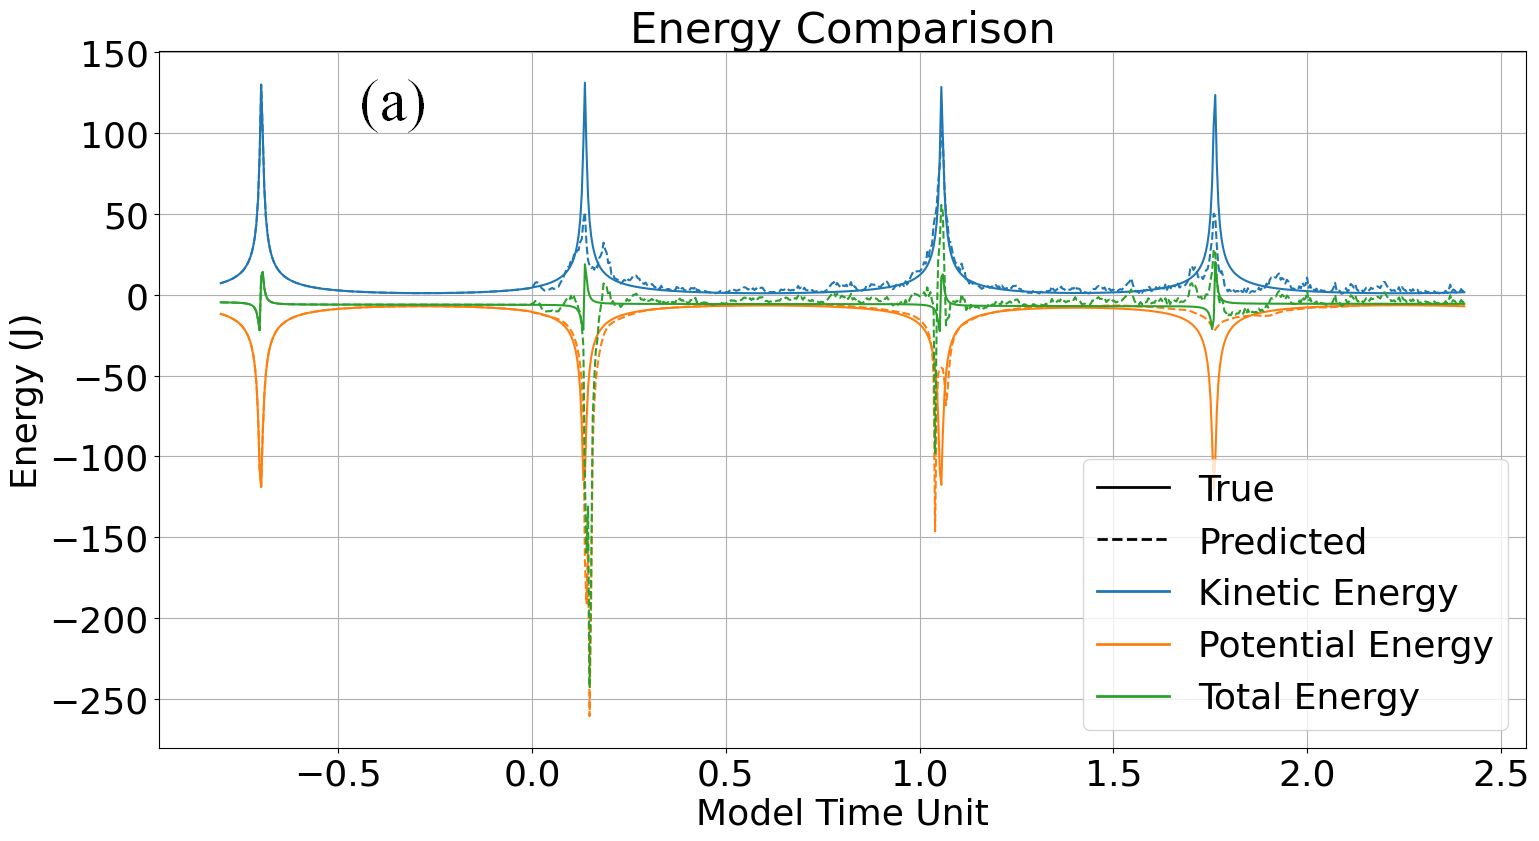
\includegraphics[width=0.497\linewidth]{plot_1_Energy_Reservoir_marked.png}
    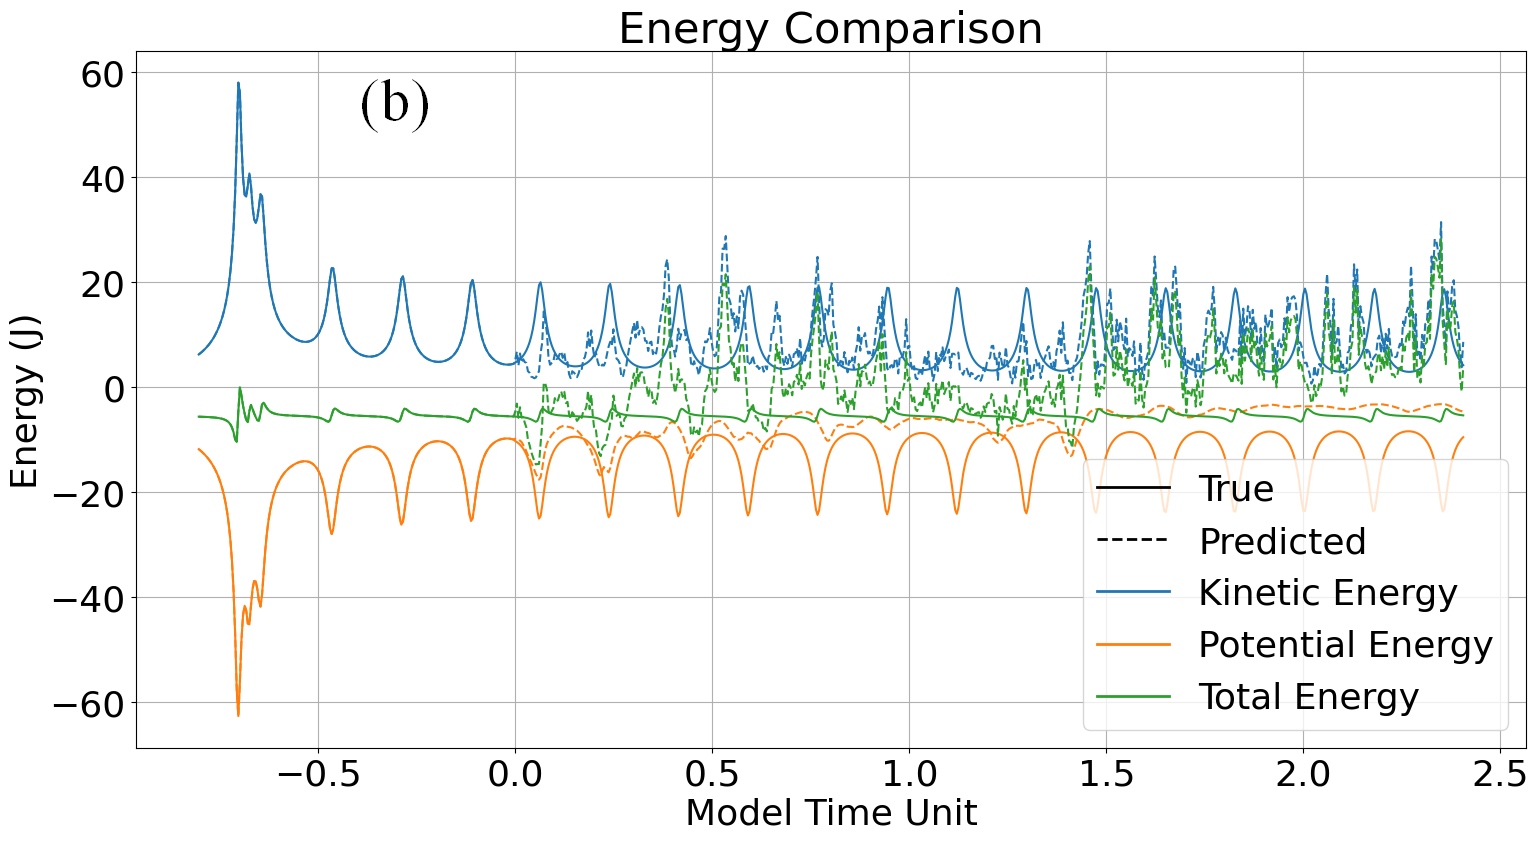
\includegraphics[width=0.497\linewidth]{plot_3_Energy_Reservoir_marked.png}
    \caption{\textbf{Energy Conservation:} In the simulation, energy is not conserved when the bodies are close to each other. The model conserves the energy to some extent.}
    \label{fig:energy}
\end{figure*}

The bodies typically had two types of behaviors; when all three bodies interacted as in figure \ref{fig:prediction_set_1_results} and when one body would do go off in its own orbit, while the other two interacted with higher frequency, as in figure \ref{fig:prediction_set_2_results}. The second type was more common, so the LSTM model would focus on learning that type of behavior, while the TCN would learn to some extent, but it was only the reservoir model that actually learned how the bodies interacted.

Surprisingly, the TCN model, despite showing higher error in the short term, eventually outperformed the reservoir model at the longest forecast horizons (above 200 time steps), indicating its potential for long-range temporal dependencies when properly tuned.

%% Commenting this out with iffalse:
\iffalse
\begin{table}
    \caption{{\bf Overview of results for different forecast horizons.} Root Mean Square Error (RMSE) for position forecasts of three models at different horizons. 
} 
    \begin{tabular}{|c|ccc|ccc|ccc|}
        \hline
        \textbf{Forecast} & \multicolumn{3}{c|}{\textbf{Reservoir}} & \multicolumn{3}{c|}{\textbf{LSTM}} & \multicolumn{3}{c|}{\textbf{TCN}} \\
        \textbf{Horizon} & \multicolumn{3}{c|}{\textbf{Model}} & \multicolumn{3}{c|}{\textbf{Model}} & \multicolumn{3}{c|}{\textbf{Model}} \\
        \textbf{(Time Steps)} & \textbf{x} && \textbf{y} & \textbf{x} && \textbf{y} & \textbf{x} && \textbf{y} \\
        \hline
        1   & 0.095 && 0.075 & 0.376 && 0.388 & 0.406 && 0.425 \\
        25  & 0.148 && 0.158 & 0.406 && 0.399 & 0.426 && 0.433 \\
        50  & 0.196 && 0.198 & 0.440 && 0.411 & 0.441 && 0.443 \\
        100 & 0.251 && 0.259 & 0.499 && 0.446 & 0.470 && 0.472 \\
        200 & 0.355 && 0.379 & 0.627 && 0.552 & 0.541 && 0.546 \\
        \hline
    \end{tabular}
    \label{tab:rmse_forecast}
\end{table}
\fi

\begin{table}[htbp]
    \centering
    \caption{Distance RMSE Results for Different Models and Forecast Horizons}
    \label{tab:distance_rmse_updated}
    \begin{tabular}{|l|c|c|c|c|c|c|}
        \hline
        \textbf{Model} & \textbf{H=1} & \textbf{H=25} & \textbf{H=50} & \textbf{H=100} & \textbf{H=200} & \textbf{H=600} \\
        \hline
        LSTM & 0.456 & 0.370 & 0.383 & 0.424 & 0.507 & 1.030 \\
        \hline
        TCN & 0.244 & 0.253 & 0.263 & 0.298 & 0.393 & 0.813 \\
        \hline
        Reservoir & 0.038 & 0.146 & 0.199 & 0.281 & 0.434 & 0.949 \\
        \hline
        Combined & 0.078 & 0.145 & 0.181 & 0.228 & 0.319 & 0.727 \\
        \hline
    \end{tabular}
\end{table}

\iffalse
\begin{table}[htbp]
    \centering
    \caption{Distance RMSE Results for Different Models and Forecast Horizons}
    \label{tab:distance_rmse}
    \begin{tabular}{|l|c|c|c|c|c|c|}
        \hline
        \textbf{Model} & \textbf{H=1} & \textbf{H=25} & \textbf{H=50} & \textbf{H=100} & \textbf{H=200} & \textbf{H=600} \\
        \hline
        LSTM & 0.865 & 0.637 & 0.616 & 0.613 & 0.683 & 1.270 \\
        \hline
        TCN & 0.355 & 0.341 & 0.355 & 0.377 & 0.466 & 0.885 \\
        \hline
        Reservoir & 0.037 & 0.158 & 0.204 & 0.265 & 0.398 & 1.002 \\
        \hline
        Combined & 0.068 & 0.144 & 0.184 & 0.232 & 0.321 & 0.728 \\
        \hline
    \end{tabular}
\end{table}
\fi

\iffalse
\begin{table}[h]
    \centering
    \caption{RMSE of Predicted Positions $(x, y)$ for Each Model Across Forecast Horizons}
    \begin{tabular}{|c|cc|cc|cc|}
        \hline
        \textbf{Horizon} & \multicolumn{2}{c|}{\textbf{Reservoir Model}} & \multicolumn{2}{c|}{\textbf{LSTM Model}} & \multicolumn{2}{c|}{\textbf{TCN Model}} \\
        \cline{2-7}
         & $x$ & $y$ & $x$ & $y$ & $x$ & $y$ \\
        \hline
        1   & 0.024 & 0.026 & 0.513 & 0.424 & 0.159 & 0.162 \\
        25  & 0.093 & 0.116 & 0.424 & 0.365 & 0.172 & 0.179 \\
        50  & 0.124 & 0.150 & 0.442 & 0.384 & 0.185 & 0.193 \\
        100 & 0.177 & 0.181 & 0.497 & 0.416 & 0.222 & 0.206 \\
        200 & 0.276 & 0.303 & 0.623 & 0.489 & 0.274 & 0.248 \\
        600 & 0.687 & 0.740 & 1.316 & 0.882 & 0.488 & 0.563 \\
        \hline
    \end{tabular}
    \label{tab:rmse_results}
\end{table}
\fi

%%% - E5 - %%%%%%%%%%%%%%%%%%%%%%%%%%%%%%%%%%%%%%




\section{\label{sec:conclusion}Conclusions and Outlook} %%% DO NOT CHANGE!

%%% - B6 - %%%%%%%%%%%%%%%%%%%%%%%%%%%%%%%%%%% 
%%% Customize this part: text between - B6 - and - E6 - must not appear in the final report 

Due to the complexity of the chaotic system with three moving objects, machine learning models had trouble predicting the outcome of the system. 
Some models showed promise in predicting the trajectories of the bodies -- especially \textbf{Reservoir models}, and to some extent also \textbf{TCN:s}. \textbf{LSTM:s} had troubles to learn anything apart from the general direction of the particles. It proved difficult to use neural network models to classify the final outcome of the system.
Future work would look closer at preserving system energy.
While model-free approaches such as reservoir computing proved most reliable overall, convolutional architectures like TCNs show promising long-term forecasting capabilities, especially when energy conservation is approximately preserved. The key challenge remains capturing the chaotic attractor without overfitting to noise or diverging due to numerical instabilities. Future work could investigate hybrid architectures, incorporate physics-informed priors, or enforce energy constraints explicitly during training to further improve generalization and physical fidelity. A method to test would be to use PINNs as in \cite{RAISSI2019686}.

\begin{itemize}
    \item Conclusions and Outlook: TCN and Reservoir outperformed the LSTM. The Reservoir was able to capture the behavior of the system while the TCN was good at capturing the general direction of the bodies. By combining those two, the system performed quite well.
    By using a smaller time step, one could make sure that the energy was conserved in the system. Physical laws could be introduced in the loss function to make sure that the trained model would behave according to physical laws. 
\end{itemize}
%%% - E6 - %%%%%%%%%%%%%%%%%%%%%%%%%%%%%%%%%%%%%%
\iffalse
\begin{table}
    \begin{center}
        \caption{\bf This is just kept as a reminder and making sure I don't exceed 5 pages.}
        \begin{tabular}{|c|c|c|c|c|c|}
        \hline
            \raisebox{0pt}[13pt][6pt]{\hspace*{3pt}} \parbox[c][][c]{1.2cm}{\textbf{Project team}} & 
            \raisebox{0pt}[13pt][6pt]{\hspace*{3pt}} \parbox[c][][c]{1.0cm}{\textbf{Pages}} & 
            \raisebox{0pt}[13pt][6pt]{\hspace*{3pt}} \parbox[c][][c]{1.2cm}{\textbf{Refs (min)}} & 
            \raisebox{0pt}[13pt][6pt]{\hspace*{3pt}} \parbox[c][][c]{1.2cm}{\textbf{Refs (max)}} & 
            \raisebox{0pt}[13pt][6pt]{\hspace*{3pt}} \parbox[c][][c]{1.2cm}{\textbf{Figs (min)}} & 
            \raisebox{0pt}[13pt][6pt]{\hspace*{3pt}} \parbox[c][][c]{1.2cm}{\textbf{Figs (max)}} 
        \\
        \hline
            \raisebox{0pt}[13pt][6pt]{\hspace*{3pt}} 1 &   5 & 5 & 10 & 3 & 6  \\   
        \hline
            \raisebox{0pt}[13pt][6pt]{\hspace*{3pt}} 2 &   9 & 10 & 20 & 5 & 9  \\   
        \hline
            \raisebox{0pt}[13pt][6pt]{\hspace*{3pt}} 3 &  13 & 15 & 30 & 7 & 11 \\       
            \hline
        \end{tabular}
    \end{center}
\end{table}
\fi


\section{\label{sec:Contribution}Contributions} %%% DO NOT CHANGE!

%%% - B7 - %%%%%%%%%%%%%%%%%%%%%%%%%%%%%%%%%%% 
%%% Customize this part: text between - B7 - and - E7 - must not appear in the final report 
The author solely wrote the manuscript and performed the data analysis. E.A. contributed to conceptualizing the project and implementing the code.

%%% - E7 - %%%%%%%%%%%%%%%%%%%%%%%%%%%%%%%%%%%%%%



\section{\label{sec:COI}Conflict of Interest} %%% DO NOT CHANGE!

%%% - B8 - %%%%%%%%%%%%%%%%%%%%%%%%%%%%%%%%%%% 
%%% Customize this part: text between - B8 - and - E8 - must not appear in the final report 
The author declares no conflict of interest.

%%% - E8 - %%%%%%%%%%%%%%%%%%%%%%%%%%%%%%%%%%%%%%




\section{\label{sec:datacode}Data and Code Availability} %%% DO NOT CHANGE!

%%% - B9 - %%%%%%%%%%%%%%%%%%%%%%%%%%%%%%%%%%% 
%%% Customize this part: text between - B9 - and - E9 - must not appear in the final report 
All code and datasets used in this project are available at: \href{https://github.com/ebsbel/threebody}{https://github.com/ebsbel/threebody}.

%%% - E9 - %%%%%%%%%%%%%%%%%%%%%%%%%%%%%%%%%%%%%%



%%% - B10 - %%%%%%%%%%%%%%%%%%%%%%%%%%%%%%%%%%% 
%%% Customize this part: text between - B10 - and - E10 - must not appear in the final report 
%%% - E10 - %%%%%%%%%%%%%%%%%%%%%%%%%%%%%%%%%%%%%%






\bibliography{biblio-TIF360-FYM360} %%% DO NOT CHANGE!
% Produces the bibliography via BibTeX.

\end{document}
